\section{GEEK Algorithm}

    \begin{figure}
        \centering
        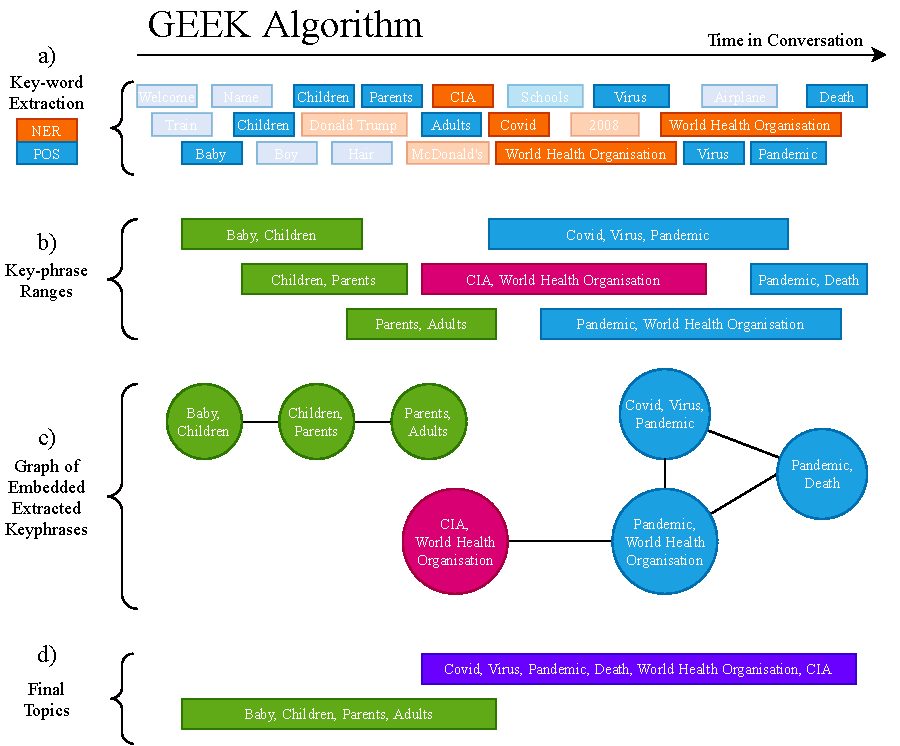
\includegraphics[width=\textwidth]{geek.pdf}
        \caption{A toy example showing how GEEK works.\newline a) \Glspl{keyphrase} are extracted as nouns and proper nouns using \gls{pos} tagging (blue) and as named entities using \gls{ner} (orange). The words on a transparent background are discarded because they are not similar to other nearby \glspl{keyphrase}.\newline b) The \glspl{keyphrase} are matched with similar nearby \glspl{keyphrase} and the range of their effect is determined. \newline c) A graph of \glspl{keyphrase} is created based on \gls{keyphrase}-range overlap and similarity. The colour is meant to serve as a visualisation of embeddings (similar colour $\rightarrow$ similar embedding).\newline
        d) The topics are the \glspl{keyphrase} in connected components in the graph. They range from the earliest \gls{keyphrase} occurence to the latest. The meaning of the final topic is influenced by all connected \glspl{keyphrase} (shown here as colour mixing).
        }
        \label{fig:geek architecture}
    \end{figure}

We use the TopicRank approach and build upon it to develop an algorithm that both segments and labels topics. We call this improved algorithm the \gls{geek}. \gls{geek} extracts \glspl{keyphrase}, but uses \glspl{embedding} to achieve a better selection than TopicRank. It then uses embedding-based similarity to determine cohesive sections of the transcript. An example of how GEEK works is shown in Fig. \ref{fig:geek architecture}.

GEEK is based on the following assumptions:

\begin{enumerate}
    \item Topics are described by a small number of \glspl{keyphrase}. We assume \glspl{keyphrase} to exclusively be nouns, proper nouns and named entities, such as \textit{family}, \textit{music}, \textit{Donald Trump, the CIA} or \textit{Tesla}.
    \item Topics are sections within the text that feature similar \glspl{keyphrase}. \glspl{keyphrase} that are only mentioned once can not represent a topic.
    \item There can be more than one active topic: topics can overlap and smaller sub-topics can be discussed within larger topics.
    \item If the gap between related \glspl{keyphrase} is too large, they do not belong to the same segment.
\end{enumerate}

    \subsection{Hyperparameters}
    The hyperparameters that the user needs to set to use \gls{geek} are as follows:

    \newcolumntype{t}{>{\hsize=.15\hsize}X}
    \newcolumntype{L}{>{\hsize=.7\hsize}X}
    \begin{table}[H]
        \centering
        \begin{tabularx}{0.9\textwidth}{| t | L | t |}
        \hline
        \textbf{Symbol} & \textbf{Description} & \textbf{Chosen Value} \\ \hline
        $\Delta_{\text{max}}$     & The maximum gap between matching \glspl{keyphrase} for them to be considered in the same segment & 11                    \\ \hline
        $\eta_{\text{min}}$     & The minimum cosine similarity of two word \glspl{embedding} for their words to be considered similar. & 0.55                        \\ \hline
        $T_{\text{min}}$ & Minimum number of \glspl{utterance} a topic must span. & 3 \\ \hline

        \end{tabularx}
    \end{table}
    

    \subsection{Keyword Extraction}
        TopicRank extracts noun phrases such as
        \begin{equation*}
            ``\textbf{The spotted puppy}\text{ is up for adoption.}",
        \end{equation*}
        as \glspl{keyphrase}. We instead only extract the nouns, proper nouns and named entities themselves (and no surrounding adjectives/articles). We do this because most multi-word noun phrases do not have pre-trained \glspl{embedding}. However, if a two-word phrase ends in a noun and is a part of the \glspl{embedding} it is also added as a \gls{keyphrase} to include phrases such as ``neural net" and ``absolute zero". The \glspl{embedding} used here are the \textit{\gls{numberbatch} mini} \gls{embedding} (which sacrifice a little bit of accuracy for much smaller filesizes). The \gls{keyphrase} extraction process is shown in Fig. \ref{fig:geek architecture} a).

        \subsubsection{POS Tagging}
            We extract \gls{pos} tags using the pre-trained state of the art \gls{pos} tagger by the python library Flair\cite{flairNLP}. It tags every word with its grammatical function and allows us to extract nouns and proper nouns (see Sec. \ref{sssec: POS tagging}).

        \subsubsection{Named Entity Recognition}
            We also use the pre-trained state of the art \gls{ner} tagger from the python library Flair\cite{flairNLP}.
            \Gls{ner} models
            \begin{equation}
              \hat{f}_{\text{ner}}: \mathcal{S} \rightarrow \mathcal{N},
            \end{equation}
            extract words $\mathcal{N}$ in sequences of words $\mathcal{S}$ that describe a named entity such as a person, company or date and label them accordingly. For example:

        \begin{align*}
        \text{[Bill Gates, founded, Microsoft, in, 1975]} \rightarrow [& (\text{Bill Gates, person}), \\
                                                                       & (\text{Microsoft, company}), \\
                                                                       & (\text{1975, year})].
        \end{align*}
        This tagging problem is also approached almost exactly like the \gls{da} tagging from Sec. \ref{ssec: da classification}. And allows us to extract named entities as \glspl{keyphrase}.

        \subsubsection{Post Processing}
            Some words are technically nouns but are unwanted as \glspl{keyphrase}. They include words such as ``dude", ``everything" or ``dope". We manually exclude 89 such words $\mathcal{W}_{man}$ from the \glspl{keyphrase} and also exclude any words that are similar enough to any $w_{man} \in \mathcal{W}_{man}$, where similarity is defined as usual as the cosine similarity of two word \glspl{embedding} and $0.9$ is the minimum cosine similarity for exclusion.

    \subsection{Determining Keyword Ranges}
        After we extract \glspl{keyphrase}, we determine the range of \glspl{utterance} over which it is ``active" (see Fig. \ref{fig:geek architecture} b)). We do this by starting at the \gls{utterance} containing a \gls{keyphrase} $u_i$ and searching the next $\Delta_{\text{max}}$ \glspl{utterance} for matches, where matches are defined as \glspl{keyphrase} whose \glspl{embedding} $\mathbf{w_i}, \mathbf{w_j}$ have a similarity
        \begin{equation}
            \text{cosine}(\mathbf{w_i}, \mathbf{w_j}) \geq \eta_{\text{min}}.
        \end{equation}
        If a match is found at \gls{utterance} $u_j$, the search is repeated with the \textbf{same \gls{keyphrase}}, this time starting from $u_j$. This is repeated until no match is found. Then the end of the range is defined to be the last occurrence of a match. If the range is smaller than $T_{\text{min}}$, the range is discarded.

    \subsection{Joining Topic Ranges}
        Now the \gls{keyphrase} ranges are joined so that similar overlapping \glspl{keyphrase} are joined. To do this, all \gls{keyphrase} ranges $k_i$ are represented as nodes in a Graph. Two nodes $k_i$ and $k_j$ are connected if $k_i$ and $k_j$ match and if the ranges of $k_i$ and $k_j$ overlap. We essentially follow the minimum cut procedure discussed in Sec. \ref{method: utterance embedding clustering}, but instead of sentences, we cluster overlapping \glspl{keyphrase}. The clustered $k_i$ represent the final topic labels, their ranges determine the final segmentation. This process is illustrated in Fig. \ref{fig:geek architecture} c) and d). An example of the final outcome (applied to a real conversation transcript) that shows many of \gls{geek}'s features is visualised in Fig. \ref{fig:GEEK final result}.

        \begin{figure}
            \centering
            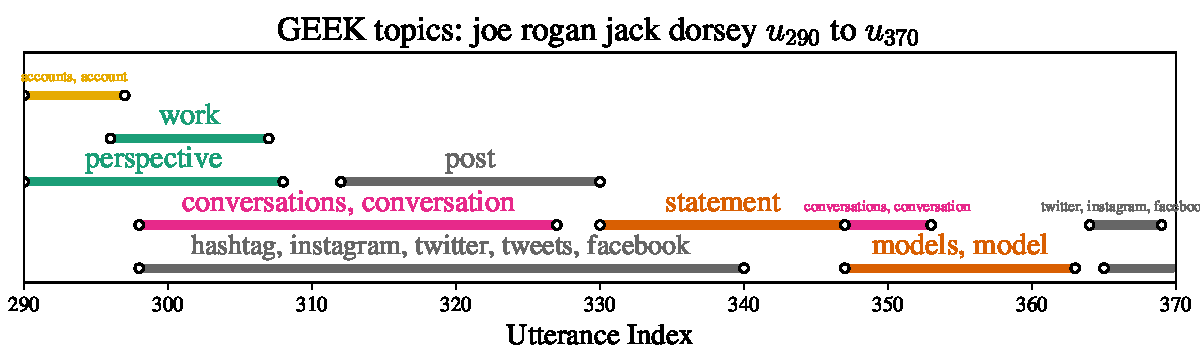
\includegraphics[width=\textwidth]{joe_rogan_jack_dorsey290_370_topics.pdf}
            \caption{An excerpt of a conversation between podcast host Joe Rogan and twitter CEO Jack Dorsey. The y-axis is used to display simultaneous topics. Similar \glspl{keyphrase} are grouped together into topics. Topics are colour-coded by mapping \glspl{embedding} to a colour.}
            \label{fig:GEEK final result}
        \end{figure}

    \subsection{Evaluation}

    \subsubsection{Segmentation}
        Even though segmentation is not exactly possible as there are multiple topics that may overlap, by simply placing a topic boundary at the start of the largest topic out of a group of overlapping topics, we can achieve a reasonable approximation. This is visualised in Fig. \ref{fig:GEEK segment}.
        \begin{figure}
             \centering
             \begin{subfigure}[b]{\textwidth}
                 \centering
                 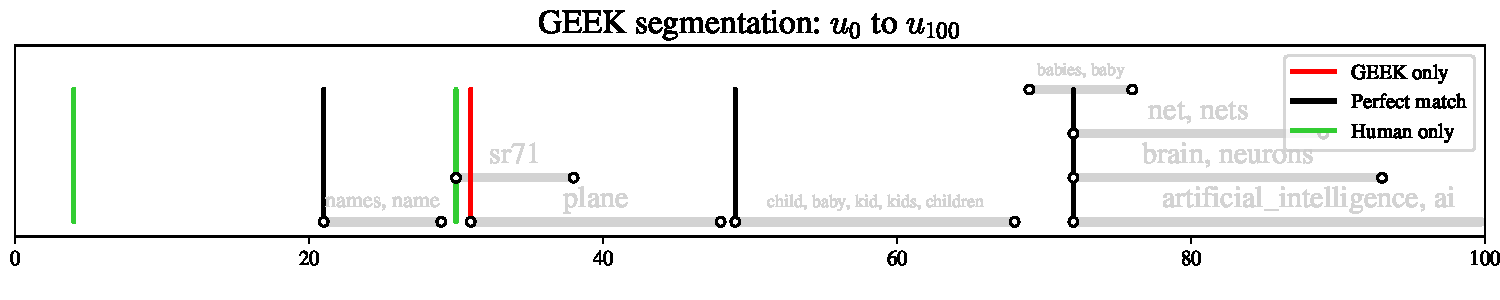
\includegraphics[width=1\textwidth]{figures/0to100segment_topics.pdf}
                 \caption{$u_0$ to $u_100$}
             \end{subfigure}
             \hfill
             \begin{subfigure}[b]{\textwidth}
                 \centering
                 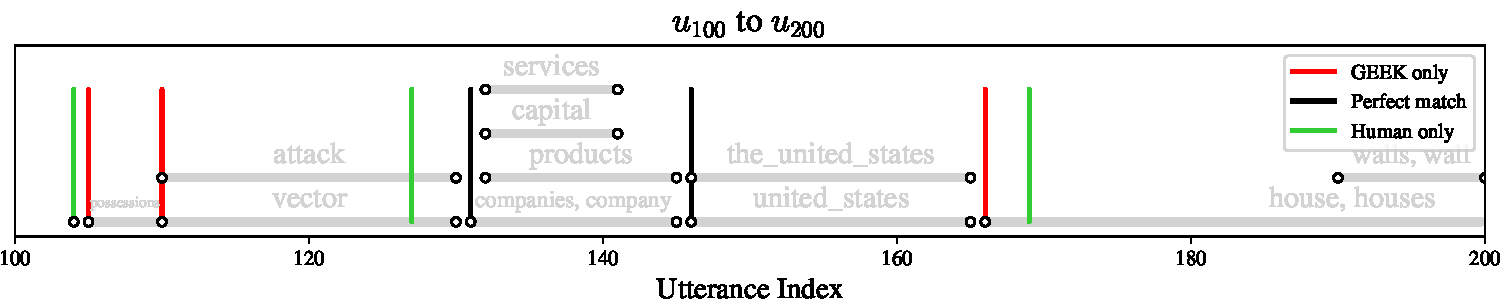
\includegraphics[width=1\textwidth]{figures/100to200segment_topics.pdf}
             \end{subfigure}
                \caption{200 \glspl{utterance} out of the evaluation transcript of a conversation between host Joe Rogan and guest Elon Musk. Vertical lines indicate boundaries: Green lines indicate human boundaries, red lines indicate boundaries placed by \gls{geek} and black lines are boundaries where the two agree exactly. Most boundaries are exactly or approximately detected by \gls{geek}. Failures include $u_4$ (missed topic change) or $u_{110}$ (false boundary).}
                \label{fig:GEEK segment}
        \end{figure}

        Using this approximation, GEEK achieves a state of the art windowDiff score of
        \begin{equation}
            w_d = 0.22 \pm 0.04.
        \end{equation}


    \subsubsection{Labelling}
        We evaluate extracted topic labels in the same way we evaluated TopicRank \glspl{keyphrase} (Sec. \ref{method: topic rank}), with the small modification that multi-word topics match if any constituent words match the human annotation. This modification is small because multi-word topics already contain very similar words. GEEK achieves an accuracy of
        \begin{equation}
            0.72 \pm 0.12,
        \end{equation}
        which is a significant improvement over TopicRank (see Eq. \ref{eq: topic rank accuracy}). It should be noted that only one author annotated selected \glspl{keyphrase}, which is a subjective task. It is expected that \gls{geek}'s accuracy is thus somewhat biased as its assumptions align more with the author's assumptions than TopicRanks's do. In future work it would be preferable to have multiple human annotators which provides an insight into labelling uncertainty and provides a more objective evaluation.

    \subsection{Limitations}
    GEEK still suffers from some limitations that are likely difficult to solve.

    \subsubsection{False Keywords}
        Some words are nouns and are used in conversation but do not describe topics. While \gls{geek} is somewhat robust against this, by requiring \glspl{keyphrase} to appear at least twice at least $T_{\text{min}}$ \glspl{utterance} apart, sometimes it fails. An example is the phrase ``attack vector" that Elon Musk uses in the conversation shown in Fig. \ref{fig:GEEK segment}. This phrase is a non-standard way of saying ``point of weakness", but because Elon Musk, and eventually the host Joe Rogan, keep using it, it is detected by \gls{geek} as two \glspl{keyphrase} ``attack" and ``vector". This leads to a wrong segmentation (the red vertical line at $u_{110})$.

    \subsubsection{Missed Topics}
        In some cases \gls{geek} also suffers from the opposite issue: minimum topic length may discard some actual topics that happen to be over quickly. An example for that is a missed boundary at $u_4$ in Fig. \ref{fig:GEEK segment}.

    \subsubsection{Ambiguous Embeddings}
        Certain matches are not detected because words can not be disambiguated (see Sec. \ref{fig:ambiguous_embedding}). For example, in Fig. \ref{fig:GEEK final result}, the \gls{keyphrase} ``post" should be included in the topic ``hasthag, instagram twitter, tweets, facebook", because ``post" and ``tweets" should be considered similar. Unfortunately, the word ``post" has ambiguous meanings, which leads to a poor embedding. To fix this, newer transformer \glspl{embedding} such as ElMo\cite{peters2018elmo} or BERT\cite{devlin2018bert}, that make \glspl{embedding} context-dependent and thus disambiguated could be evaluated in future work. \newline
